\documentclass{standalone}
\usepackage{tikz}

\begin{document}
\usetikzlibrary{positioning,shapes,arrows,snakes}
\definecolor{yellowish}{HTML}{FFE699}
\definecolor{grayish}{HTML}{D9D9D9} 
\tikzset{
   rect/.style={
      align=center,
      text=black,    
      minimum width=2.5cm,
      minimum height=2cm}
}
\tikzset{
   done/.style={rect, fill=grayish }
}
\tikzset{
   todo/.style={rect, fill=yellowish}
}
\tikzset{
   arrow/.style={line width=1mm}
}
\centering

\begin{tikzpicture}[font=\sffamily\Large\bfseries]
   \node[anchor=south west,inner sep=0](image) at (0,0) {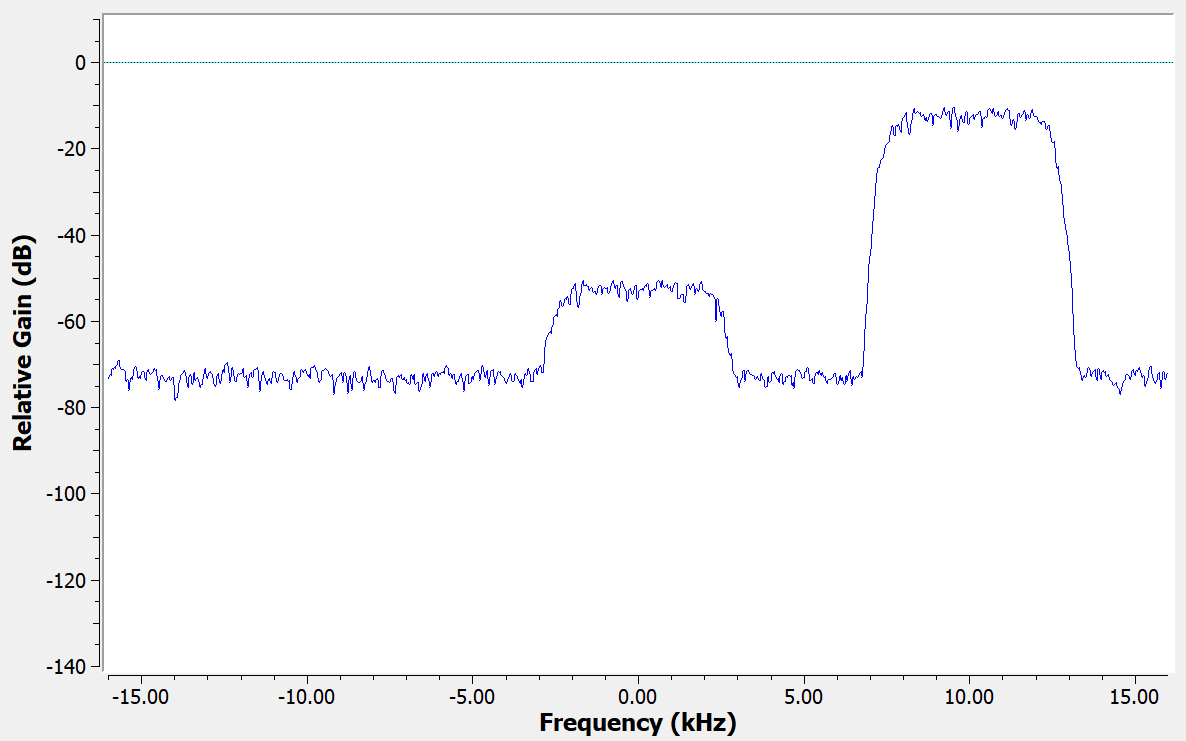
\includegraphics[scale=0.7]{filter_use_case_nolabel.png}};
   \begin{scope}[x={(image.south east)},y={(image.north west)}]
      \draw[red, ->] (0.3, 0.7) node[above left, align=center]{Gewenste\\signaal} -- (0.45, 0.6);
      \draw[red, ->] (0.9, 0.8) node[above right, align=center]{Ongewenst\\signaal} -- (0.8, 0.7);
      \draw[red, ->] (0.25, 0.2) node[below, align=center]{Ruisvloer} -- (0.3, 0.4);      
   \end{scope}
\end{tikzpicture}
\end{document}